\documentclass{article}
\usepackage{qilin}
\tikzstyle{process} = [rectangle, rounded corners, minimum width=1.5cm, minimum height=0.5cm,align=center, draw=black, fill=gray!30, auto]
\title{AER372: Control Systems  \\ Assignment 3}
\author{QiLin Xue}
\date{Spring 2023}

\usepackage{empheq}
\newcommand*\widefbox[1]{\fbox{\hspace{2em}#1\hspace{2em}}}

\usepackage{mathrsfs}
\usetikzlibrary{arrows}
\usepackage{stmaryrd}
\usepackage{accents}
\newcommand{\ubar}[1]{\underaccent{\bar}{#1}}
\usepackage{pgfplots}
% \numberwithin{equation}{section}
\usepackage{amsmath, amssymb, graphics, setspace}

\newcommand{\mathsym}[1]{{}}
\newcommand{\unicode}[1]{{}}
\usepackage{tabu}
\newcounter{mathematicapage}
\usepackage[numbered,framed]{matlab-prettifier}

\usepackage{filecontents}
\begin{filecontents*}{q6_manual.m}
%%% Define the transfer function
% kp(1+a/s) = kp s + a*kp / s
kp=45.049;
alpha=0.5;
beta=0.17;

C = tf([kp*beta kp kp*alpha],[1 0]);
G = tf(1, [1 6 5]);
sys = G*C/(1+G*C);

%%% Get Step Input Result
step_sys = feedback(sys, 1);
step_info = stepinfo(step_sys);

% Simulate the response to a step input
t = 0:0.01:20;
y = step(sys, t);

% Calculate the steady-state error
steady_state_value_step = y(end);
input_mag_step = 1;

%%% Get Ramp Input Result
% Simulate the response to the ramp input
t = 0:0.1:10;
ramp_input = t;
[y, t] = lsim(sys, ramp_input, t);

% Calculate the steady-state error
steady_state_value = y(end);
input_mag = max(ramp_input);

disp("DS1: Step SS Error="+abs(steady_state_value_step - input_mag_step)/input_mag_step)
disp("DS2: Ramp SS Error="+abs(steady_state_value - input_mag)/input_mag)
disp("DS3: Overshoot="+step_info.Overshoot)
disp("DS4: Settling time="+step_info.SettlingTime)
\end{filecontents*}

\begin{filecontents*}{q6_auto.m}
% Define the criteria
DS1_target = 0.01;
DS2_target = 0.28;
DS3_target = 5;
DS4_target = 1.5;

% Define the parameter ranges
kp_range = 10:1:30;
alpha_range = 0.5:0.05:1.3;
beta_range = 0.05:0.01:0.2;

% Initialize the minimum kp and the minimum DS4
min_kp = Inf;
min_alpha = Inf;
min_Beta = Inf;
% Loop over all possible combinations of kp, alpha, and beta
for kp = kp_range
    for alpha = alpha_range
        for beta = beta_range
            % Calculate the DS1, DS2, DS3, and DS4
            [DS1, DS2, DS3, DS4] = calculate_DS(kp, alpha, beta);
            
            % Check if the criteria are satisfied and update the minimum
            if DS1 < DS1_target && DS2 < DS2_target && DS3 < DS3_target && DS4 < DS4_target
                    if min([kp kp*alpha kp*beta]) < min([min_kp min_kp*min_alpha min_kp*min_beta])
                        min_kp = kp;
                        min_alpha = alpha;
                        min_beta = beta;
                    end
            end
        end
    end
end

% Print the minimum kp and minimum DS4
if min_kp == Inf
    disp("No combination of parameters satisfies the criteria.")
else
    disp("Minimum kp: " + min_kp)
    disp("Minimum alpha: " + min_alpha)
    disp("Minimum beta: "+ min_beta)
end

[DS1, DS2, DS3, DS4] = calculate_DS(min_kp, min_alpha, min_beta)
\end{filecontents*}

\begin{filecontents*}{function.m}
function [DS1, DS2, DS3, DS4] = calculate_DS(kp, alpha, beta)
    % Define the transfer function
    C = tf([kp*beta kp kp*alpha],[1 0]);
    G = tf(1, [1 6 5]);
    sys = G*C/(1+G*C);

    % Get Step Input Result
    step_sys = feedback(sys, 1);
    step_info = stepinfo(step_sys);
    t = 0:0.01:20;
    y = step(sys, t);

    % Calculate the steady-state error for step input
    steady_state_value_step = y(end);
    input_mag_step = 1;

    % Get Ramp Input Result
    t = 0:0.1:10;
    ramp_input = t;
    [y, t] = lsim(sys, ramp_input, t);

    % Calculate the steady-state error for ramp input
    steady_state_value = y(end);
    input_mag = max(ramp_input);

    % Return DS1, DS2, DS3, and DS4 as outputs
    DS1 = abs(steady_state_value_step - input_mag_step)/1;
    DS2 = abs(steady_state_value - input_mag)/1;
    DS3 = step_info.Overshoot;
    DS4 = step_info.SettlingTime;
end
\end{filecontents*}
\let\ph\mlplaceholder % shorter macro
\lstMakeShortInline"

\lstset{
  style              = Matlab-editor,
  basicstyle         = \mlttfamily,
  escapechar         = ",
  mlshowsectionrules = true,
}

\begin{document}

\maketitle
\begin{enumerate}[label=\textbf{3.\arabic*}]
\item We want to turn the characteristic equation into the form $a(s) + L(s)b(s)$ where $a(s),b(s)$ are monic polynomials. We have:
\begin{enumerate}[label=(\alph*)]
    \item We have the characteristic polynomial
    \begin{equation}
        (s+c)^3 + A(Ts+1)=0.
    \end{equation}
    \begin{enumerate}[label=(\roman*)]
        \item Versus parameter A: We can rewrite 
        \begin{equation}
            (s+c)^3 + AT(s+1/T)=0.
        \end{equation}
        Therefore,
        \begin{equation}
            \boxed{a(s) = (s+c)^3,\qquad b(s) = s+1/T,\qquad  L(s) = \frac{s+1/T}{(s+c)^3}}
        \end{equation}
        \item Versus parameter T: We can rewrite 
        \begin{equation}
            (s+c)^3 + A + ATs.
        \end{equation}
        Therefore,
        \begin{equation}
            \boxed{a(s) = (s+c)^3 + A,\qquad b(s) = s,\qquad  L(s) = \frac{s}{(s+c)^3 + A}}.
        \end{equation}
        \item Versus parameter $c:$ This is impossible since the characteristic equation contains nonlinear terms in $c$. However, it is still possible to find the roots of the characteristic equation. We can use the cubic equation,
        \begin{equation}
            c = \omega^k\sqrt[3]{-A(ts+1)}-s
        \end{equation}
        for $k=0,1,2$ and $\omega$ is the principal 3rd root of unity. Alternatively (and more realistically), we can use a more superior computer algebra system such as Mathematica to find the roots.
        \begin{center}
            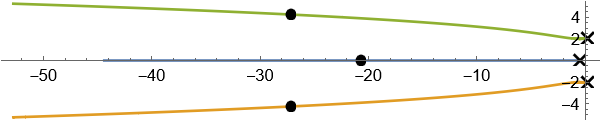
\includegraphics[width=0.7\linewidth]{A3_imgs/q1aiii.png}
        \end{center}
    \end{enumerate}
    \item We have 
    \begin{equation}
        1 + \left[k_P + \frac{k_I}{s} + \frac{k_Ds}{\tau s + 1}\right]A \frac{c(s)}{d(s)} = 0.
    \end{equation}
    \begin{enumerate}[label=(\roman*)]
        \item Versus $k_P:$ We rewrite
        \begin{equation}
            \left(1 + \left[\frac{k_I}{s} + \frac{k_Ds}{\tau s + 1}\right] A \frac{c(s)}{d(s)}\right) + k_P A \frac{c(s)}{d(s)}=0.
        \end{equation}
        To make everything a polynomial, we multiply by $d(s)s(\tau s + 1)$ to get 
        \begin{align}
            &\left(d(s)s(\tau s + 1) + A (k_{D} s^{2} + k_{I} (s \tau + 1)) c{(s)}\right) + k_P A c(s) s(\tau s + 1)=0.
        \end{align}
        The highest degree is in the term $s^2 \tau d(s)$ since $d$ has a higher degree than $c(s).$ Then dividing by $\tau,$ we have 
        \begin{align}
            &\left(d(s)s(s + 1/\tau) + A (k_{D} s^{2}/\tau + k_{I} (s + 1/\tau)) c{(s)}\right) + k_P A c(s) s(s + 1/\tau)=0 \\ 
            \implies & \left(s^{2} d{(s)}+\frac{s d{(s)}}{\tau} + \frac{A k_{D} s^{2} c{(s)}}{\tau} + A k_{I} s c{(s)} + \frac{A k_{I} c{(s)}}{\tau}\right) + k_P A c(s) (s^2 + s/\tau) = 0.
        \end{align}
        Therefore, 
        \begin{empheq}[box=\widefbox]{align}
            a(s) &= s^{2} d{(s)}+\frac{s d{(s)}}{\tau} + \frac{A k_{D} s^{2} c{(s)}}{\tau} + A k_{I} s c{(s)} + \frac{A k_{I} c{(s)}}{\tau} \\ 
             b(s) &= c(s)(s^2+s/\tau) \\ 
             L(s) &= = \frac{s (s \tau + 1) c{(s)}}{s d{(s)} + \tau (A k_{I} s c{(s)} + d{(s)}) + A k_{D} s^{2} c{(s)} + A k_{I} c{(s)}}
        \end{empheq}
        \item Versus $k_I:$ Same thing but make the substitution $k_P \gets \frac{k_I}{s}$ and $k_I \gets k_Ps.$ This gives 
        \begin{align}
            &\left(s^{2} d{(s)}+\frac{s d{(s)}}{\tau} + \frac{A k_{D} s^{2} c{(s)}}{\tau} + A k_Ps^2 c{(s)} + \frac{A k_P s c{(s)}}{\tau}\right) + k_I A c(s) (s + 1/\tau) = 0.
        \end{align}
        Which gives 
        \begin{empheq}[box=\widefbox]{align}
            a(s) &= s^{2} d{(s)}+\frac{s d{(s)}}{\tau} + \frac{A k_{D} s^{2} c{(s)}}{\tau} + A k_Ps^2 c{(s)} + \frac{A k_P s c{(s)}}{\tau} \\ 
            b(s) &=c(s) (s + 1/\tau)  \\ 
            L(s) &= \frac{(s \tau + 1) c{(s)}}{s^{2} \tau d{(s)} + s d{(s)} + A k_{D} s^{2} c{(s)} + A k_{P} s^{2} \tau c{(s)} + A k_{P} s c{(s)}}
        \end{empheq}
        \item Versus $k_D$: We can rewrite 
        \begin{align}
            &\left(s^{2} d{(s)}+\frac{s d{(s)}}{\tau} + \frac{A k_{D} s^{2} c{(s)}}{\tau} + A k_{I} s c{(s)} + \frac{A k_{I} c{(s)}}{\tau}\right) + k_P A c(s) (s^2 + s/\tau) = 0 \\ 
            \implies & \left(s^{2} d{(s)}+\frac{s d{(s)}}{\tau} + A k_{I} s c{(s)} + \frac{A k_{I} c{(s)}}{\tau} + k_P A c(s) (s^2 + s/\tau)\right) + k_{D}\frac{A s^{2} c{(s)}}{\tau} = 0.
        \end{align}
        This gives
        \begin{empheq}[box=\widefbox]{align}
            a(s) &= s^{2} d{(s)}+\frac{s d{(s)}}{\tau} + A k_{I} s c{(s)} + \frac{A k_{I} c{(s)}}{\tau} + k_P A c(s) (s^2 + s/\tau) \\ 
            b(s) &= \frac{A s^{2} c{(s)}}{\tau} \\ 
            L(s) &= \frac{A s^{2} c{(s)}}{s^{2} \tau d{(s)} + s d{(s)}+A k_{I} s \tau c{(s)} + A k_{I} c{(s)} + A k_{P} s^{2} \tau c{(s)} + A k_{P} s c{(s)}}
        \end{empheq}
        \item Versus $\tau:$ We can rewrite, multiply by $\tau$, and then collect terms
        \begin{align}
            &\left(s^{2} d{(s)}+\frac{s d{(s)}}{\tau} + \frac{A k_{D} s^{2} c{(s)}}{\tau} + A k_{I} s c{(s)} + \frac{A k_{I} c{(s)}}{\tau}\right) + k_P A c(s) (s^2 + s/\tau) = 0 \\ 
            \implies & A k_{D} s^{2} c{(s)} + A k_{P} s c{(s)} + A k_{I} c{(s)}+ s d{(s)} + A k_{I} s \tau c{(s)} +  A k_{P} s^{2} \tau c{(s)}  + s^{2} \tau d{(s)}  = 0 \\ 
            \implies & \left(A k_{D} s^{2} c{(s)} + A k_{P} s c{(s)} + A k_{I} c{(s)}+ s d{(s)}\right) + \tau\left(A k_{I} s  c{(s)} +  A k_{P} s^{2}  c{(s)}  + s^{2}  d{(s)}\right) = 0.
        \end{align}
        Dividing by $Ak_D$ gives 
        \begin{align}
            \left(s^{2} c{(s)} + \frac{k_{I} c{(s)}}{k_{D}} + \frac{k_{P} s c{(s)}}{k_{D}} + \frac{s d{(s)}}{A k_{D}}\right) + \frac{\tau}{Ak_D}\left(A k_{I} s  c{(s)} +  A k_{P} s^{2}  c{(s)}  + s^{2}  d{(s)}\right) = 0.
        \end{align}
        This gives 
        \begin{empheq}[box=\widefbox]{align}
            a(s) &=s^{2} c{(s)} + \frac{k_{I} c{(s)}}{k_{D}} + \frac{k_{P} s c{(s)}}{k_{D}} + \frac{s d{(s)}}{A k_{D}} \\ 
            b(s) &= A k_{I} s  c{(s)} +  A k_{P} s^{2}  c{(s)}  + s^{2}  d{(s)} \\ 
            L(s) &= Ak_D \frac{s^{2} d{(s)} + A k_{I} s c{(s)} + A k_{P} s^{2} c{(s)}}{A k_{D} s^{2} c{(s)} + A k_{I} c{(s)} + A k_{P} s c{(s)} + s d{(s)}}.
        \end{empheq}
    \end{enumerate}
\end{enumerate}
\item \begin{enumerate}[label=(\alph*)]
    \item Note that $G(s)$ has $m=0$ roots and has $n=3$ poles, particularly 
    \begin{equation}
        s=0, s = -2 \pm i.
    \end{equation}
    \textbf{Asymptotes:} The number of asymptotes is $n-m=3$ with angles 
    \begin{equation}
        \phi_\ell = \frac{180^\circ + 360^\circ (\ell-1)}{3} = \boxed{60^\circ, 180^\circ, -60^\circ}
    \end{equation}
    for $\ell = 1,2,3,$ and they radiate from the point on the real line,
    \begin{equation}
        \alpha =  \frac{0+(-2+i)+(-2-i)}{3} = \boxed{-\frac{4}{3}}.
    \end{equation}
    \textbf{Breakaway and Break-in Points:} They occur when $1+G(s)$ hits a local minimum/maximum (i.e. a saddle-node bifurcation like behaviour), which leads to when $\frac{dL(s)}{ds}=0.$ We can compute,
    \begin{equation}
        \frac{d}{ds}\left(s^3+4s^2+5s\right) = 3 s^{2} + 8 s + 5 =0 \implies \boxed{ s = - \frac{5}{3}, \  s = -1}
    \end{equation}
    \textbf{Angles of departure and arrival:} The angle of departure of the pole $-2+i$ is given by 
    \begin{align}
        \phi_\text{dep} &= -\sum_{i\neq \text{dep}} \phi_i - 180^\circ \\ 
        &= -\left((180^\circ-\tan^{-1}(1/2)) + 90^\circ\right)-180^\circ \\ 
        &= \boxed{-63.43^\circ}.
    \end{align}
    The angle of departure of the pole $-2-i$ is given by 
    \begin{align}
        \phi_\text{dep} &= -\sum_{i\neq \text{dep}} \phi_i - 180^\circ \\ 
        &= -\left((180^\circ+\tan^{-1}(1/2)) - 90^\circ\right)-180^\circ \\ 
        &= \boxed{63.43^\circ}.
    \end{align}
    The angle of departure of the pole $0$ is given by 
    \begin{align}
        \phi_\text{dep} &= -\sum_{i\neq \text{dep}} \phi_i - 180^\circ \\ 
        &= -(180^\circ - \tan^{-1}(1/2) + 180^\circ + \tan^{-1}(1/2))-180^\circ \\ 
        &= \boxed{180^\circ}.
    \end{align}
    There are no angles of arrival since the system has no zeros.

    \textbf{Crossings with imaginary axis:} For what values of $K$ does $1+G(s)$ have roots that are purely imaginary? We have,
    \begin{equation}
        1 + G(s) =0 \implies s^3+4s^2+5s+K=0.
    \end{equation}
    Substituting $s=bi,$ we have
    \begin{equation}
        -b^3i-4b^2+5bi+K=0.
    \end{equation}
    We want the real and the imaginary part to be zero, i.e. this gives the system 
    \begin{align}
        K&=4b^2 \\
        5b&=b^3 
    \end{align}
    We get $b=0,\pm\sqrt{5},$ so we get $K=0,20.$ At $K=0$ the roots cross the imaginary axis at $s=0$ and at $K=20$ the roots cross the imgainary axis at $\boxed{s=\pm \sqrt{5}i}.$

    I draw the plot below,
    \begin{center}
        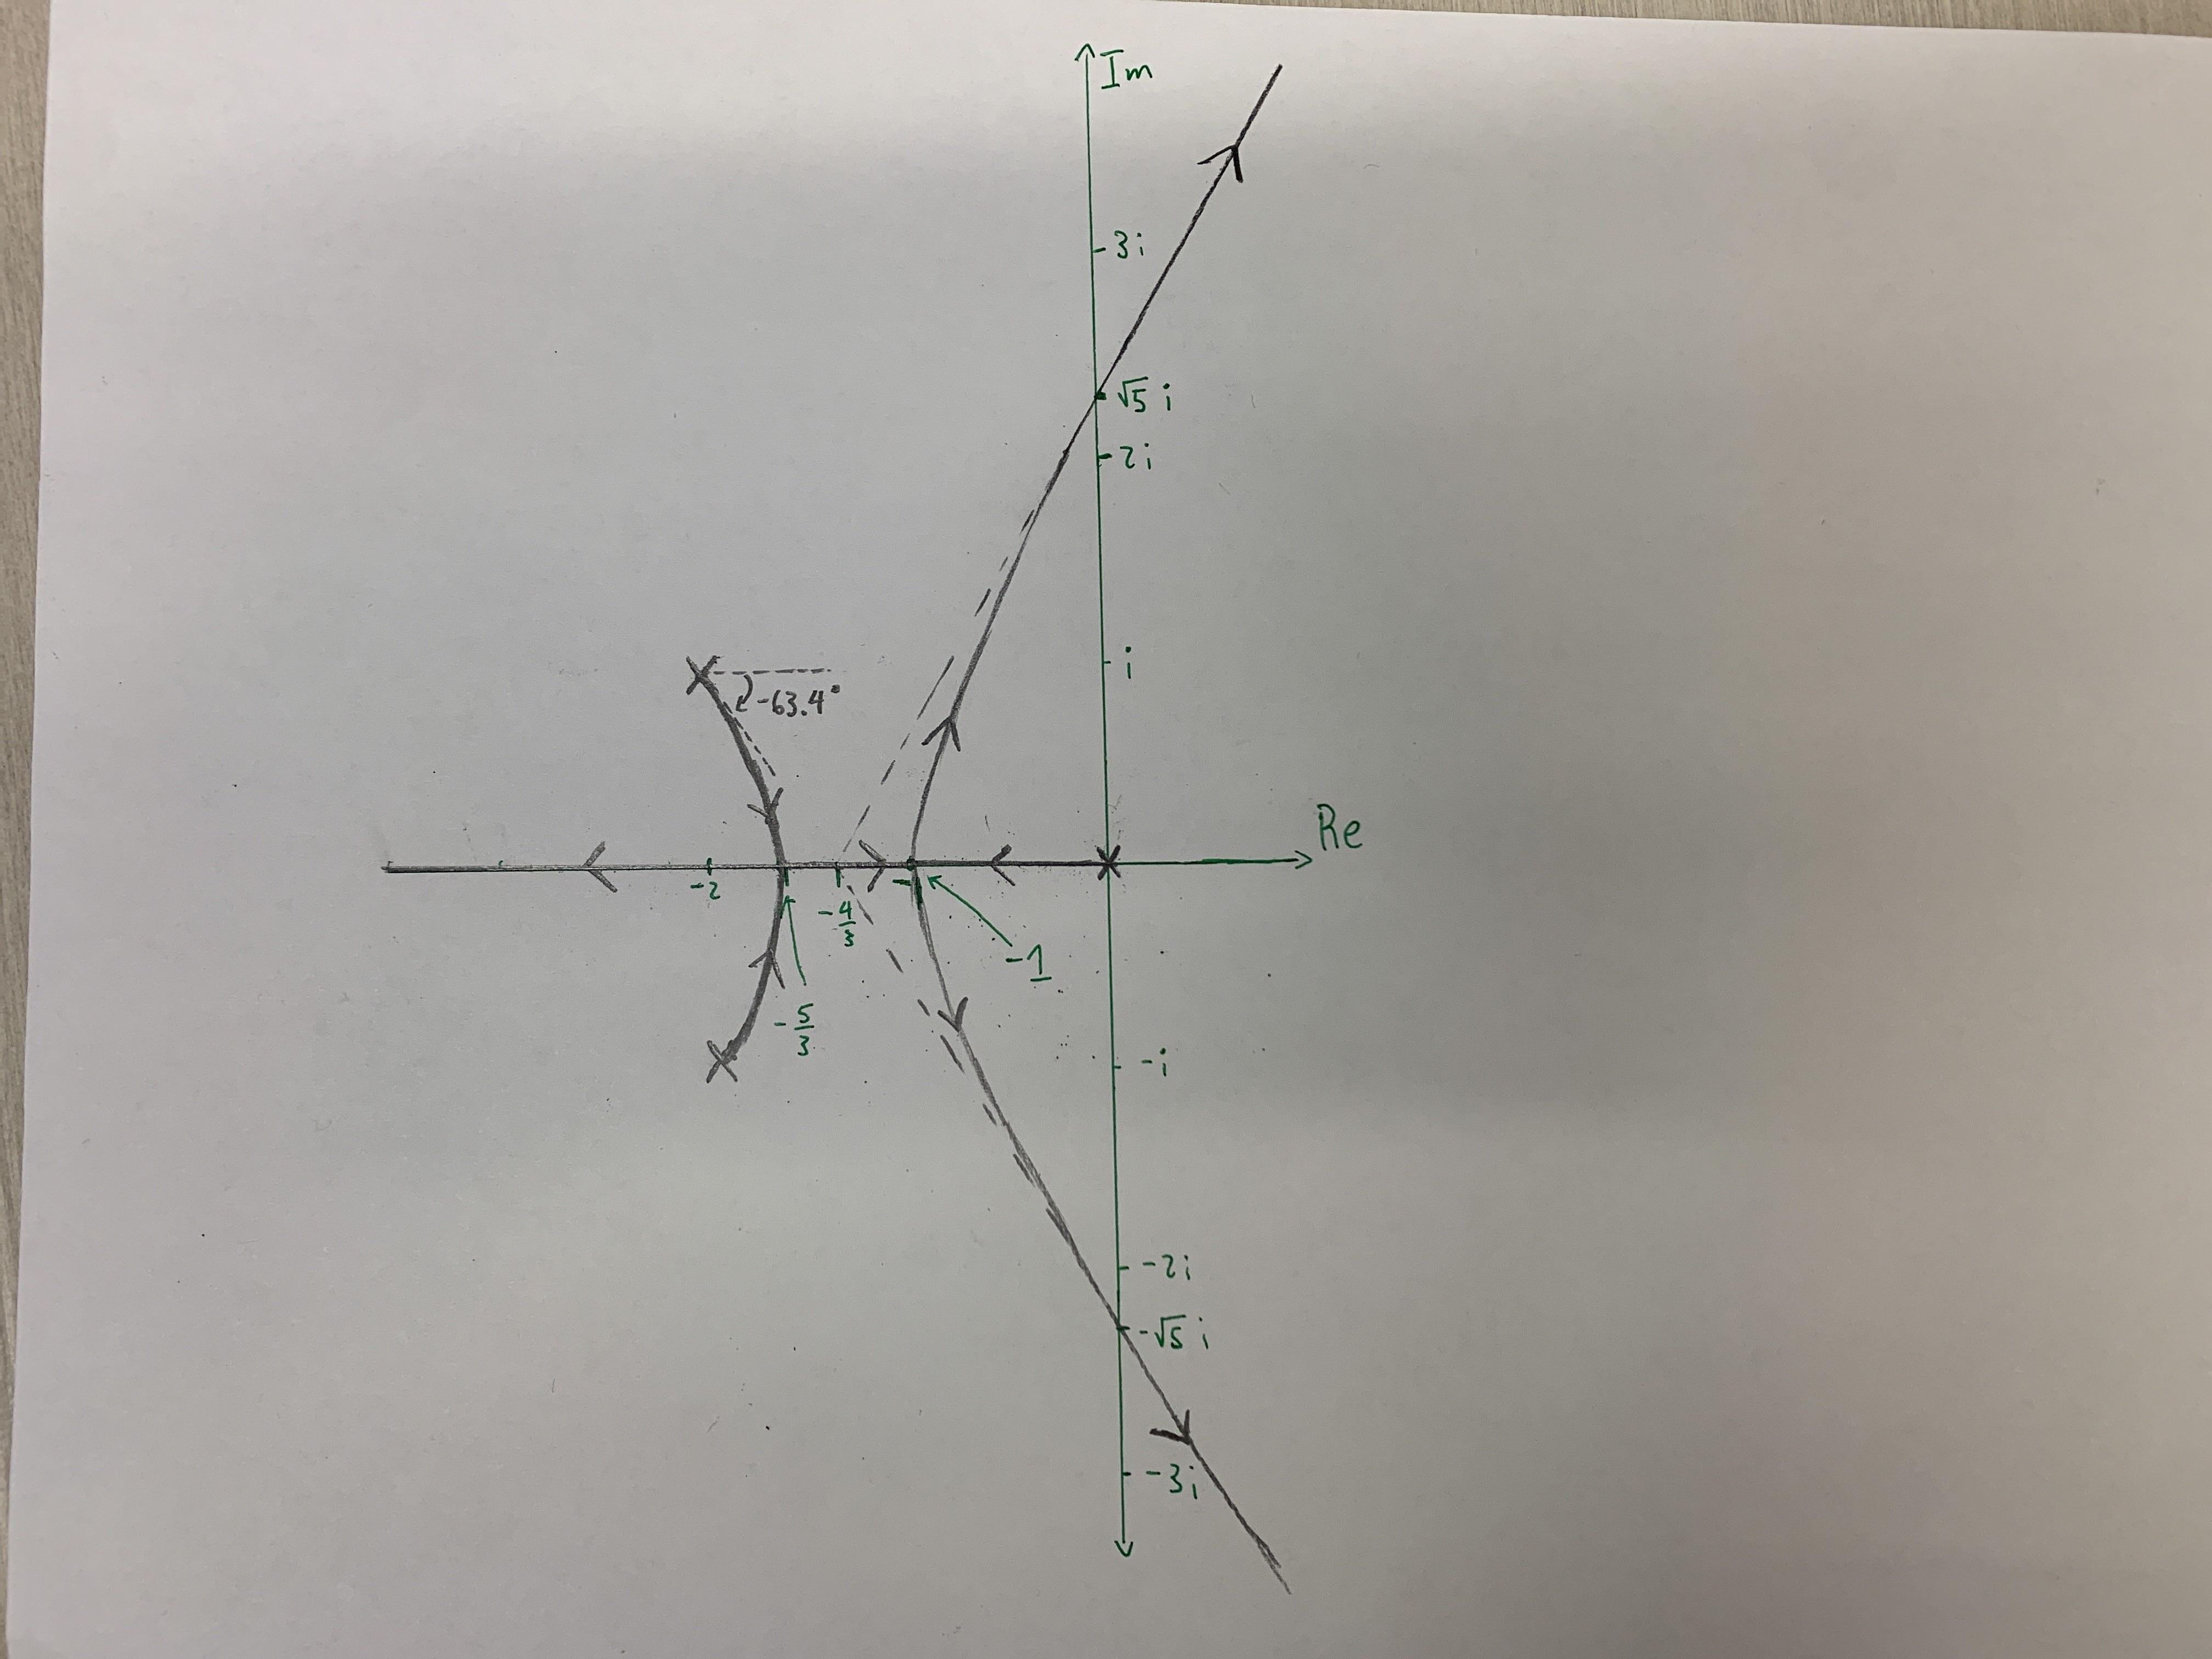
\includegraphics[width=\linewidth]{A3_imgs/q2.jpg}
    \end{center}
    where the arrows indicate the direction the roots are moving with increasing $K.$ I used Matlab to verify these results.
    \item The system is underdamped when the roots have negative real parts (so it's stable) and a nonzero imaginary part (so it's oscillatory). Similarly, the system is overdamped when the roots have negative real parts with a zero imaginary part. When they transition, we have critical damping, which occurs at $s=-1,-5/3.$ We just need to find the corresponding $K$ value.
    
    Recall that $1+G(s) =0 \implies s^3+4s^2+5s+K=0.$ Then Plugging in $s=-1$ gives 
    \begin{equation}
        (-1)^3+4(-1)^2+5(-1)+K = K - 2 =0 \implies \boxed{K=2},
    \end{equation}
    and 
    \begin{equation}
        (-5/3)^3+4(-5/3)^2+5(-5/3)+K  = K - \frac{50}{27} =0 \implies \boxed{K \approx 1.85}.
    \end{equation}
    Before $K=1.85,$ we have two roots (which originated from $-2\pm i$) have a nonzero imaginary part and after $K=2,$ we have one root (which originated from $s=0$ with a nonzero imaginary part). Therefore:
    \begin{itemize}
        \item $K<1.85$ is underdamped
        \item $1.85<K<2$ is overdamped
        \item $2<K<20$ is underdamped.
    \end{itemize}
    Beyond $K=20$ it passes the imaginary axis, so it becomes unstable.
\end{enumerate}
\item For the three cases, we have the following root-locus plots:
\begin{center}
    (a)
    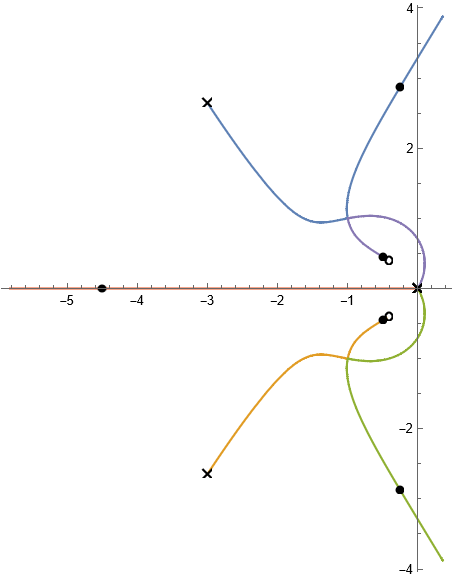
\includegraphics[width=0.4\linewidth]{A3_imgs/q3a.png}
    (b)
    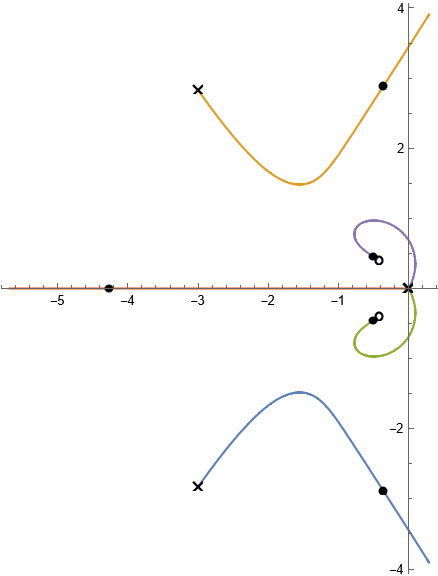
\includegraphics[width=0.4\linewidth]{A3_imgs/q3b.png}
    
    \vspace{2mm}
    (c)
    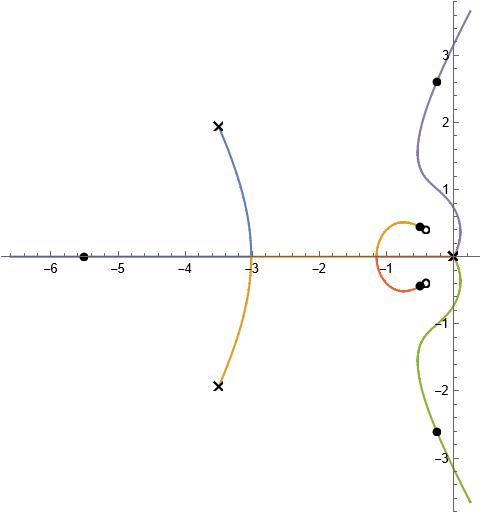
\includegraphics[width=0.4\linewidth]{A3_imgs/q3c.png}
\end{center}
To analyze these plots, we perform some basic computations. First, the zeros occur at 
\begin{equation}
    s^2+(5/6)s+(1/3)=0 \implies  s = - \frac{5}{12} \pm \frac{\sqrt{23} i}{12}
\end{equation}
which corresponds to the two open circles in the plots, i.e. these are where two of the roots will end up as $K\to \infty.$ For all three plots, there are five poles, one at $s=0$ with multiplicity $3$ (so there are three branches coming out) and two poles $s,\bar{s}$ with a negative real part and a non-zero imaginary component. These are represented by an X. We compare the plots pairwise:
\begin{itemize}
    \item (a) and (b): The breakaway points for part (a) are 
    \begin{equation}
        s = -1 \pm i, -1.56 \pm 0.497i
    \end{equation}
    The second pair of breakway points do not lie on the locus, but $-1 \pm i$ does, so we have an intersection point between two branches. However, for (b), the breakaway points are 
    \begin{equation}
        s = -1.14 \pm 0.976i, -1.42 \pm 0.716i.
    \end{equation}
    Here, the real component of the breakaway point has changed slightly, due to modifying the constant term in the denominator. This slight change has made the breakaway point not lie on the locus, so we do not have an intersection point between two branches. Even if we set $\beta = 0.001$ we still have this behaviour.
    \item (a)/(b) and (c)
    The major difference here is that there are now two break-away points. We can compute the breakaway points to be
    \begin{equation}
        s=-3.02, -1.15, -0.807 \pm 0.943 i.
    \end{equation}
    Here, the conjugate roots are not on the locus, so we do not have an intersection somewhere off the real-axis. However, there are still two intersection points between branches on the real axis, specifically at $-3.02$ and $-1.15.$ This means that the other poles and zeros (excluding $s=0$) need to have a branch that crosses this point and connects it to the real-axis.
\end{itemize}
Note that all computations here were performed with CAS via Mathematica, along with the plots.

\item \textbf{Solution 1 (Hand computation)} Our goal is to find the poles of the closed-loop transfer function. Recall that 
\begin{equation}
    \zeta = \cos\theta \implies \theta = 60^\circ
\end{equation}
and 
\begin{equation}
    \frac{\Im s}{\Re s} = \pm \tan \theta = \pm \sqrt{3}.
\end{equation}
In other words, we want $s = -\beta + \sqrt{3}\beta i$ to be a root. Our open-loop transfer function is
\begin{equation}
    G(s)D_c(s) = \frac{10(s+a)}{s(s+1)(s+8)}
\end{equation}
and the closed-loop transfer function is
\begin{align}
    \frac{G(s)D_c(s)}{1+G(s)D_c(s)} &= \frac{\frac{10(s+a)}{s(s+1)(s+8)}}{1+\frac{10(s+a)}{s(s+1)(s+8)}} \\ 
    & = \frac{10 (a + s)}{10 a + s (s + 1) (s + 8) + 10 s}.
\end{align}
Substituting in $s=\beta+\sqrt{3}\beta i$ to the characteristic equation gives
\begin{align}
   & 10 a + (-\beta+\sqrt{3}\beta i) (-\beta+\sqrt{3}\beta i + 1) (-\beta+\sqrt{3}\beta i + 8) + 10 (-\beta+\sqrt{3}\beta i) = 0 \\
  \implies &10 a + 8 \beta^{3} - 18 \beta^{2} - 18 \sqrt{3} i \beta^{2} - 18 \beta + 18 \sqrt{3} i \beta = 0.
\end{align}
Separating into real and imaginary gives 
\begin{align}
    0 &=10a + 8\beta^3 - 18\beta^2 - 18\beta \\ 
    0 &= -18\sqrt{3} \beta^2 + 18\sqrt{3} \beta.
\end{align}
The second equation gives $\beta = 0,1.$ Plugging this into the first equation gives 
\begin{align}
    a &= \frac{-8(1)^3+18(1)^2+18(1)}{10} = 2.8 \\ 
    a &= \frac{-8(0)^3+18(0)^2+18(0)}{10} = 0.
\end{align}
Note that $a=0$ is not a valid choice, as it gives $s=0$ which does not have $\zeta=0.5.$ However, $\boxed{a=2.8}$ is valid, and is the only choice that gives a pole at $s=-\beta \pm \sqrt{3}\beta i.$

\textbf{Solution 2 (Root Locus):} The characteristic equation is
\begin{align}
    & 1 + G(s)D_c(s) = 0 \\ 
    \implies & 1 + \frac{10}{s(s+1)} \cdot \frac{s+a}{s+8} = 0 \\ 
    \implies &  10 a + s^{3} + 9 s^{2} + 18 s= 0
\end{align}
which can be put in the form of 
\begin{equation}
    (s^3+9s^2+18s) + a(10),
\end{equation}
so we can use the root-locus method on 
\begin{equation}
    \frac{10}{s^3+9s^2+18s},
\end{equation}
which gives us the following plot on Matlab:
\begin{center}
    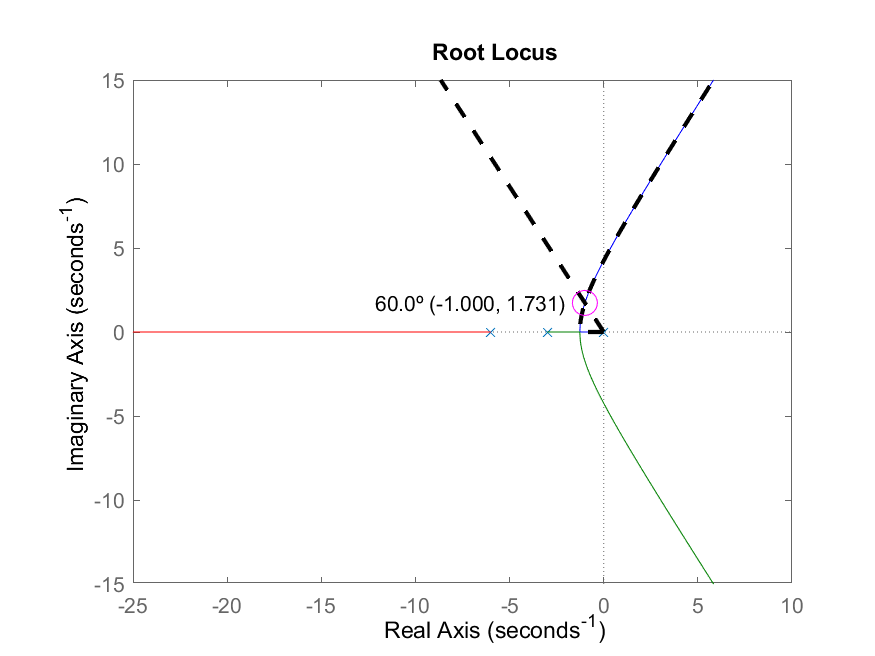
\includegraphics[width=0.7\linewidth]{A3_imgs/intersect.png}
\end{center}
where using the intersect tool, gives $a = 2.8$ as well. Note that I borrowed code from \href{https://www.mathworks.com/matlabcentral/answers/1442099-how-to-find-the-intersection-a-root-locus-plot-and-a-line-with-specific-angle}{Adam Danz} from MathWorks to get the intersection working.
\item \begin{enumerate}[label=(\alph*)]
    \item This is impossible. Refer to the root locus plot below for $KG(s).$
    \begin{center}
        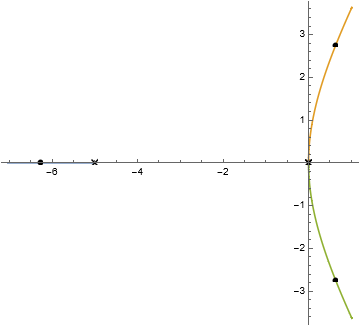
\includegraphics[width=0.5\linewidth]{A3_imgs/q5a.png}
    \end{center}
    For any $K>0$ there are two roots with a positive real part, which is unstable.
    \item The open loop gain is 
    \begin{equation}
        K \cdot \frac{1/(s^2(s+5))}{1+K_ts \cdot 1/(s^2(s+5))} = \frac{K}{s (K_{t} + s (s + 5))}.
    \end{equation}
    This has no zeros, and has poles at $s=0$ and when $s^2+5s+K_t=0,$ which occurs at 
    \begin{equation}
        s = -\frac{5}{2} \pm \frac{\sqrt{25-4K_t}}{2}.
    \end{equation}
    For $0<K_t < 25/4,$ we have the two roots $s_+,s_- < 0.$ The angle of departure from the $s=0$ root is 
    \begin{equation}
        \phi_\text{dep} = -(180^\circ + 180^\circ)-180^\circ = 180^\circ.
    \end{equation}
    Similarly, for $K_t > 25/4,$ we have two roots $s,\bar{s}$ with a negative real part and a non-zero imaginary component. The angle of departure from the $s=0$ root is still $180^\circ$ (similar computation as Q2). Finally, we should expect the same behavior at $K_t=25/4$ because we should expect the locus to change continuously as a function of $K_t.$

    Because the angle of departure is $180^\circ,$ for small values of $K$ we can guarantee that all roots have a negative real component. However, for large enough $K$ we could still have roots that go off to have a positive real component, so yes, we should expect a relation between $K$ and $K_t$ to guarantee a stable response.
    \item We have already computed some of these ranges:
    \begin{itemize}
        \item $0<K_t < 25/4$: all roots lie on the real axis with negative real part
        \item $K_t =25/4:$ there are only two distinct roots (where one has a multiplicity of $2$), both on the real axis with negative real part
        \item $25/3 > K_t > 25/4:$ there are two roots with a negative real part and a non-zero imaginary component. We will see where the $25/3$ comes from later.
    \end{itemize}
    Note that $s=0$ is a root for all of them. Also, we can compute where the break-away points are:
    \begin{equation}
        \frac{d}{ds}\left( sK_t + s^3 + 5s^2\right) = K_{t} + 3 s^{2} + 10 s = 0 \implies s = - \frac{5}{3} \pm \frac{\sqrt{25 - 3 K_{t}}}{3}.
    \end{equation}
    For $K_t < \frac{25}{3},$ there are two distinct breakaway points. But at $K_t = 25/3$ there is only one, and as $K_t > 25/3$ there are none, signifying a change in behaviour. This gives two more regions:
    \begin{itemize}
        \item $K_t = \frac{25}{3}:$ there is one breakaway point
        \item $K_t > \frac{25}{3}:$ there are no breakaway points.
    \end{itemize}
    \item No overshoot occurs when the system is critically or over-damped, i.e. the poles are on the negative real axis (so not oscillations). The rise time is determined by how far away the poles are from the imaginary axis. Because of this, we will look for when this root has a multiplicity of $2$ (i.e. if it didn't, then one root would always be to the right (and to the left) of this double root, so a local min/max can only exist at a double root).
    
    Note that these are the poles of the closed-loop system, which are the roots of 
    \begin{equation}
        s^3 + 5s^2 + K_ts + K =0.
    \end{equation}
    The double root can only occur when the derivative is zero, i.e.
    \begin{equation}
        3s^2 + 10s + K_t \implies s = - \frac{5}{3} \pm \frac{\sqrt{25 - 3 K_{t}}}{3} 
    \end{equation}
    but since $K_t\le 5$ is the upper bound, we will choose $K_t=5$ which gives $s=-5/3 \pm \sqrt{10}{3},$ i.e. $s=-0.613,-2.73.$ We can plug these values back into the original equation to get the corresponding $K$ values:
    \begin{align}
        &(-0.613)^3+5(-0.613)^2+5(-0.613)+K = 0 \implies K = 1.416501397 \\ 
        &(-2.73)^3+5(-2.73)^2+5(-2.73)+K = 0 \implies K = -3.268083
    \end{align}
    so only the first value is valid since $K>0.$ Thus, we pick 
    \begin{equation}
        \boxed{(K_t,K) = (5,1.4)}.
    \end{equation}
    We can plot this in MATLAB,
    \begin{center}
        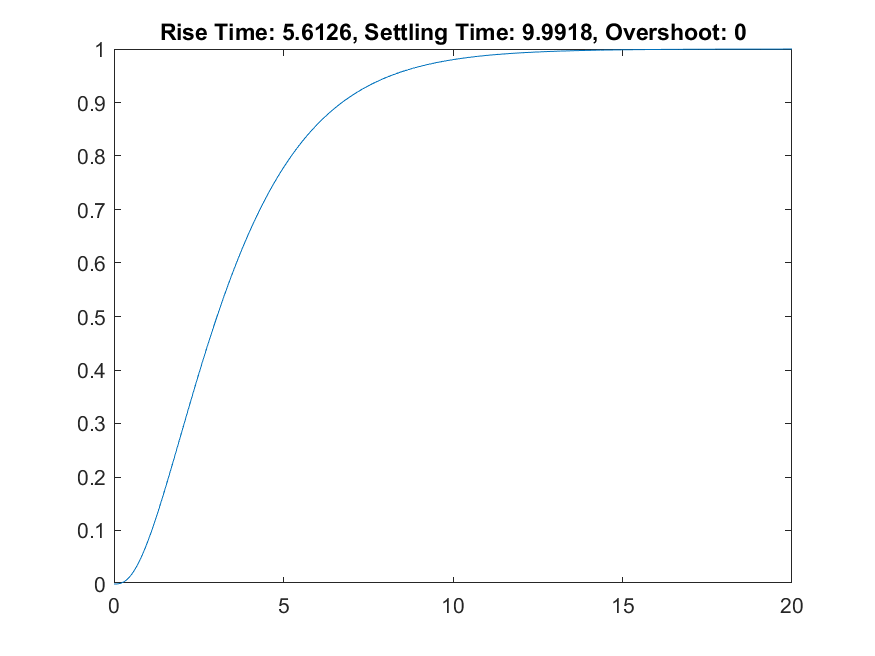
\includegraphics[width=0.8\linewidth]{A3_imgs/A3_q5_step.png}
    \end{center}
    \item Using MATLAB, I was able to make the root-locus plot for the open-loop transfer function 
    \begin{equation}
        \frac{K}{s^3+5s^2+5s}
    \end{equation}
    where $K_t=5$ was used. This value was used because of the earlier discussion of how increasing $K_t$ will cause the rise time to increase. The plot is shown below,
    \begin{center}
        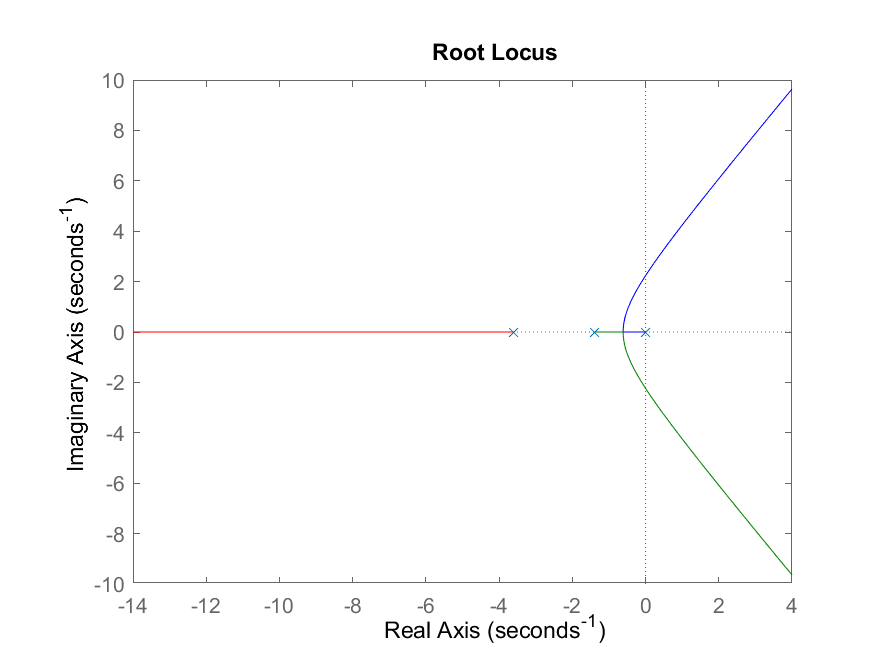
\includegraphics[width=0.8\linewidth]{A3_imgs/q5_e.png}
    \end{center}
    Using \verb#rlocfind()#, we can determine the location of the breakaway point (i.e. when the system changes from overdamped to underdamped) and get around 
    \begin{equation}
        \boxed{K=1.42},
    \end{equation}
    which agrees with our earlier analysis. To verify this, we can try a few different values for $K_t,$ and we will see that this is maximized at $K_t=5.$ 
\end{enumerate}
\item Let's translate the design specifications into more useful quantities.
\begin{itemize}
    \item DS1: System needs to be type 1, i.e. have a pole at $s=0.$ This means we should have an integrator.
    \item DS2: We want $1/K_v < 0.28$ or equivalently
    \begin{equation}
        \lim_{s\to 0}sGD_{cl}(s) > 3.57.
    \end{equation}
    \item DS3: We use the equation for percent overshoot (note that here it is approximate, but we will use it as a starting point)
    \begin{equation}
        e^{-\pi \zeta/\sqrt{1-\zeta^2}} < 0.05 \implies \zeta > 0.752
    \end{equation}
    This corresponds to an angle $\theta=\cos^{-1}0.752 = 41.218^\circ,$ and 
    \begin{equation}
        \left|\frac{\Im s}{\Re s}\right| =  \tan\theta <  0.876
    \end{equation}
    \item DS4: The real part should be smaller than $-4/1.5 \approx -2.7.$
\end{itemize}
Consider a controller in the form of 
\begin{equation}
    k_P(1+\alpha/s)
\end{equation}
where $\alpha = k_I/k_P.$ We guess the poles (nice numbers that satisfy DS3,DS4) 
\begin{equation}
    s = -3 \pm 2 i
\end{equation}
in order to satisfy DS3 and DS4. Using root-locus and a bit of trial and error, we were able to obtain the poles $-2.71 \pm 1.77 i$ with $\alpha=0.7$ and $k_P=8.5938.$ To ensure it satisfies DS2, we can compute 
\begin{equation}
    \lim_{s\to 0} s \cdot 8.5938(1+0.7/s)\cdot \frac{1}{(s+1)(s+5)} = \lim_{s\to 0}\frac{8.5938 \cdot 0.7 \cdot (2 s + 1)}{(s + 1) (s + 5)} = 1.2,
\end{equation}
which is almost three times smaller than $3.57$ Repeated experimentation leads us to believe that the location of viable roots cannot change significantly by changing $k_P,\alpha,$ so we look into a three parameter controller, such as a PID controller. We have the ansatz
\begin{equation}
    k_P(1+\alpha/s+\beta s)
\end{equation}
where $\beta = k_D/k_P.$ The condition for DS2 becomes 
\begin{equation}
    \lim_{s\to 0} s k_P(1+\alpha/s+\beta s) \cdot \frac{1}{(s+1)(s+5)} = \lim_{s\to 0}\frac{k_{P} (\alpha + s (\beta s + 1))}{(s + 1) (s + 5)} = \frac{\alpha k_{P}}{5}
\end{equation}
which is the same condition as before. If we set $\alpha=0.5$ to a more ``safe'' value, then we need $k_P>35.7.$

Guessing $\beta=0.17$ with root-locus allows us to pick the roots $-6.58 \pm 0.2356i$ with $k_P=45.05,$ which meets DS2. Therefore, our proposed values are 
\begin{equation}
    \boxed{k_P = 45.05, k_I = 22.53, k_D = 7.66}.
\end{equation}
As a quick sanity check, we need to make sure the system is stable. The plant is given by 
\begin{equation}
    G(s) = \frac{1}{s^2+6s+5}
\end{equation}
so $\omega_n = \sqrt{5}, \zeta = 3/\sqrt{5} = 1.34,$ and $K=1/5.$ Routh's Stability Criterion gives
\begin{equation}
    \frac{(2\zeta+k_DK\omega_n)(1+k_PK)\omega_n}{K} = \frac{(2*1.34+7.55*1/5*\sqrt{5})(1+45.05*1/5)\sqrt{5}}{1/5} = 677.8 > k_I,
\end{equation}
so the system is stable.

The corresponding root-locus plot (for documentation purposes) is 
\begin{center}
    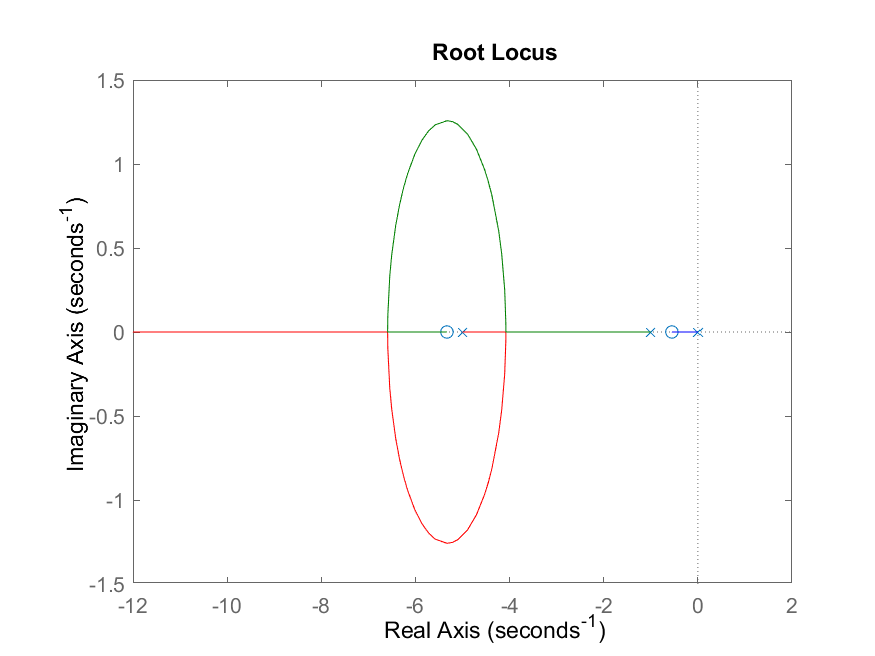
\includegraphics[width=0.8\linewidth]{A3_imgs/A3_q6_locus.png}
\end{center}
Note that at the root around $-6.6 \pm 0.2i,$ there is a third root on the real-axis near $s=0.$ We are able to ignore this pole, because it cancels out one of the zeros from the controller. This is allowed behavior since we are not cancelling out any zeros from the plant, only the controller.

\lstinputlisting[caption = {Code to Compute Design Specifications}]{q6_manual.m}

which gives us 
\begin{verbatim}
DS1: Step SS Error=1.7317e-06
DS2: Ramp SS Error=0.22137
DS3: Overshoot=0
DS4: Settling time=0.40168
\end{verbatim}
so everything is satisfied. Note that this is not the only solution. I can run a grid search algorithm to find the best solution within a certain region:
\lstinputlisting[caption = {Code to Perform Grid Search on Design Specifications}]{q6_auto.m}
which gives us
\begin{verbatim}
Minimum kp: 19
Minimum alpha: 0.95
Minimum beta: 0.1
DS1 = 1.1769e-11
DS2 = 0.2770
DS3 = 4.7056
DS4 = 0.9436
\end{verbatim}
We can compute
\begin{equation}
    \frac{k_p\alpha}{5} = 3.61 > 3.57
\end{equation}
as desired. Therefore, the optimal solution in this range is 
\begin{equation}
    \boxed{(k_p, k_I, k_D) = (19, 18.05, 1.9)}.
\end{equation}
where we are optimizing for smaller gains, which although give the same behaviour, is desired in real applications because there is less noise and it is more robust when actually implementing it (i.e. smaller voltages). Similarly, the system is stable since
\begin{equation}
    \frac{(2\zeta+k_DK\omega_n)(1+k_PK)\omega_n}{K} = \frac{(2*1.34+1.9*1/5*\sqrt{5})(1+19*1/5)\sqrt{5}}{1/5} = 189> k_I,
\end{equation}
so this is stable as well.

The function \verb#calculate_DS(kp, alpha, beta)# is defined via the following code:
\lstinputlisting[caption = {Function to Compute Design Specifications}]{function.m}
For transparency, GPT4 was used to assist in generating the grid search optimization.
\end{enumerate}

\end{document}


